\subsection{Caso de uso 1: Iniciar sesión} \label{cu1}
\subsubsection{Resumen}
Este caso de uso le permite al actor ingresar al sistema proporcionando su nombre de usuario y contraseña para poder realizar las funciones correspondientes a su perfil.
\subsubsection{Descripción}
\begingroup
\setlength{\LTleft}{-10cm plus -1fill}
\setlength{\LTright}{\LTleft}
\begin{center}  
  \captionof{table}{Caso de uso 1: Iniciar sesión } \label{tab:cu1_tab}
  \begin{longtable}{| p{3.5cm} | p{11.5cm} |}
      	\hline
      		\textbf{Versión} &  0.1 \\
        \hline 
       		\textbf{Autor} & Juan Gerardo Diaz Rodarte\\
        \hline
          \textbf{Estatus} & Edición \\
        \hline  
          \textbf{Fecha de último estatus} &  3 de abril de 2017 \\
        \hline
      \multicolumn{2}{|c|}{\large{Atributos}} \\
        \hline
          \textbf{Actor}  & Administrador, Usuario y Sub-Usuario. \\
        \hline	
          \textbf{Propósito} & Permite a los diferentes actores ingresar al sistema. \\
        \hline
          \textbf{Disparador} & El actor abre la aplicación y presiona el botón de Iniciar sesión. \\
        \hline	
          \textbf{Entradas} & 
            \begin{itemize}
              \item \textbf{Correo electrónico}: Se escribe con el teclado.
              \item \textbf{Contraseña}: Se escribe con el teclado.
            \end{itemize} \\
        \hline	
          \textbf{Salidas} & 
            \begin{itemize}
              \item \textbf{Interna}: Se redirecciona a la vista de inicio IU.
            \end{itemize} \\
        \hline	
          \textbf{Precondiciones}& 
            \begin{itemize}
              \item \textbf{Interna:} El actor debe estar registrado en el sistema.
            \end{itemize} \\
        \hline	
          \textbf{Postcondiciones} & 
            \begin{itemize}
              \item \textbf{Interna:} Al actor se le otorgan permisos para realizar actividades de acuerdo a su perfil y es redireccionado. 
		\begin{itemize}
			\item El Administrador sera redireccionado al IU Index.
			\item Para el Usuario y Sub-Usuario se redireccionara al IU Index.
		\end{itemize}
            \end{itemize} \\
       \hline
         \textbf{Reglas de negocio} & 
         	\begin{itemize}
         	  \item \textbf{\ref{rnl_01}}
         	  \item \textbf{\ref{rnl_02}}
         	  \item \textbf{\ref{rnrv_01}}
         	  \item \textbf{\ref{rnrv_02}}
         	  \item \textbf{\ref{rnrv_03}}
	 \end{itemize} \\
       \hline
         \textbf{Mensajes} & 
         	\begin{itemize}
         	  \item \textbf{\ref{msja_01}}
         	  \item \textbf{\ref{msje_01}}
         	  \item \textbf{\ref{msje_02}}
	 \end{itemize} \\
       \hline
         \textbf{Tipo} & Primario \\
    \hline	    
  \end{longtable}
\end{center}
\endgroup

\subsubsection{Trayectorias del caso de uso}
\textbf{Trayectoria principal}
\begin{enumerate}
  \item {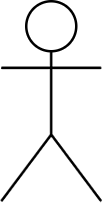
\includegraphics[scale=.1]{Capitulo3/img/actor.png} Ingresa el actor a la aplicación móvil, en el caso del administrador ingresa al portal web mediante una dirección eletrónica.}
  \item {
\includegraphics[scale=.05]{Capitulo3/img/proceso.png} Se muestar la vista IU Index para el administrador y IU Principal para los demás actores.}
  \item {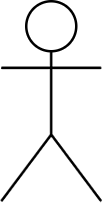
\includegraphics[scale=.1]{Capitulo3/img/actor.png} Presiona el botón de Iniciar sesión.}
  \item {
\includegraphics[scale=.05]{Capitulo3/img/proceso.png} Se redirecciona a la vista IU Iniciar sesión.}
  \item {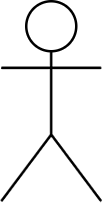
\includegraphics[scale=.1]{Capitulo3/img/actor.png} Ingresa el la dirección de correo electrónico y contraseña en los campos correspondientes.}
  \item {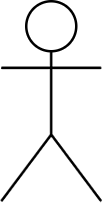
\includegraphics[scale=.1]{Capitulo3/img/actor.png} Presiona el botón para solicitar ingresar al sistema.}
  \item {
\includegraphics[scale=.05]{Capitulo3/img/proceso.png} Verifica que el usuario haya ingresado la información requerida como establecido en la \textbf{\ref{rnl_01}}. \hyperref[cu1_ta_a]{[Trayectoria alternativa A]}}
  \item {
\includegraphics[scale=.05]{Capitulo3/img/proceso.png} Verifica que la dirección de correo eletrónico y la contraseña sean válidos de acuerdo a las reglas de negocio correspondientes. \hyperref[cu1_ta_b]{[Trayectoria alternativa B]} \hyperref[cu1_ta_c]{[Trayectoria alternativa C]}}
  \item {
\includegraphics[scale=.05]{Capitulo3/img/proceso.png} Verifica que la dirección de correo eletrónico y la contraseña coincidan con aquellos datos registrados en el sistema. \hyperref[cu1_ta_d]{[Trayectoria alternativa D]} \hyperref[cu1_ta_e]{[Trayectoria alternativa E]}}
  \item {
\includegraphics[scale=.05]{Capitulo3/img/proceso.png} Se muestra la vista de hogar correspondiente al actor.}
  \item {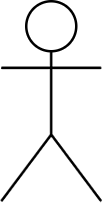
\includegraphics[scale=.1]{Capitulo3/img/actor.png} Hacer uso del sistema.}\\
  \textit{Fin de caso de uso} \\	
\end{enumerate}

\textbf{Trayectoria alternativa A} \phantomsection\label{cu1_ta_a} \\
\textbf{Condición:} El actor no proporcionó la información requerida, rompiendo la regla de negocio \textbf{\ref{rnl_01}}.\\
 \begin{enumerate}[label=A\arabic*]
    \item {
\includegraphics[scale=.05]{Capitulo3/img/proceso.png} Muestra el mensaje \textbf{\ref{msja_01}}, indicando que el actor ha dejado campos en blanco.}
    \item {Continua en el paso 5 de la trayectoria principal.} \\
    \textit{Fin de trayectoria} \\
\end{enumerate}

\textbf{Trayectoria alternativa B} \phantomsection\label{cu1_ta_b}\\
\textbf{Condición:} El actor no ingreso una dirección de correo electrónico que cumpla con la regla de negocio \textbf{\ref{rnrv_02}}.\\
 \begin{enumerate}[label=B\arabic*]
    \item {
\includegraphics[scale=.05]{Capitulo3/img/proceso.png} Muestra el mensaje \textbf{\ref{msje_02}}, indicando que la dirección de correo electrónico no es válida.}
    \item {Continua en el paso 5 de la trayectoria principal.} \\
    \textit{Fin de trayectoria} \\
\end{enumerate}

\textbf{Trayectoria alternativa C} \phantomsection\label{cu1_ta_c}\\
\textbf{Condición:} El actor ingreso una contraseña incorrecta que no cumple con la regla de negocio \textbf{\ref{rnrv_03}}.\\
 \begin{enumerate}[label=C\arabic*]
    \item {
\includegraphics[scale=.05]{Capitulo3/img/proceso.png} Muestra el mensaje \textbf{\ref{msje_01}}, indicando que el actor ha ingresado datos incorrectos.}
    \item {Continua en el paso 5 de la trayectoria principal.} \\
    \textit{Fin de trayectoria} \\
\end{enumerate}

\textbf{Trayectoria alternativa D} \phantomsection\label{cu1_ta_d}\\
\textbf{Condición:} No se encontró alguna cuenta relacionada con la dirección de correo electrónico ingresada de acuerdo a la regla de negocio \textbf{\ref{rnrv_01}}.\\
 \begin{enumerate}[label=D\arabic*]
    \item {
\includegraphics[scale=.05]{Capitulo3/img/proceso.png} Muestra el mensaje \textbf{\ref{msje_01}}, indicando que el actor ha ingresado datos incorrectos en alguno de los campos.}
    \item {Continua en el paso 5 de la trayectoria principal.} \\
    \textit{Fin de trayectoria} \\
\end{enumerate}

\textbf{Trayectoria alternativa E} \phantomsection\label{cu1_ta_e}\\
\textbf{Condición:} La contraseña ingresada no corresponde a la cuenta de la dirección de correo electrónico ingresada de acuerdo a la regla de negocio \textbf{\ref{rnrv_01}}.\\
 \begin{enumerate}[label=E\arabic*]
    \item {
\includegraphics[scale=.05]{Capitulo3/img/proceso.png} Muestra el mensaje \textbf{\ref{msje_01}}, indicando que el actor ha ingresado datos incorrectos en alguno de los campos.}
    \item {Continua en el paso 5 de la trayectoria principal.} \\
    \textit{Fin de trayectoria} \\
\end{enumerate}

\textbf{Trayectoria alternativa F} \phantomsection\label{cu1_ta_f}\\
\textbf{Condición:} El actor selecciono la opción de \textit{¿Has olvidado tu contraseña?}.\\
 \begin{enumerate}[label=F\arabic*]
    \item {
\includegraphics[scale=.05]{Capitulo3/img/proceso.png} Se ejecuta el \hyperref[cu1_1]{CU 1.1 Recuperar contraseña}} \\
    \textit{Fin de trayectoria} \\
\end{enumerate}

\textbf{Trayectoria alternativa G} \phantomsection\label{cu1_ta_g}\\
\textbf{Condición:} El actor selecciono la opción de \textit{¿Eres nuevo aquí?}.\\
 \begin{enumerate}[label=G\arabic*]
    \item {
\includegraphics[scale=.05]{Capitulo3/img/proceso.png} Se ejecuta el \hyperref[cu2]{CU 2 Registrarse}} \\
    \textit{Fin de trayectoria} \\
\end{enumerate}

\subsubsection{Puntos de extensión}
\noindent \textbf{Causa de la extensión:} El actor, de tipo de Usuario o Sub-Usuario, selecciono \textit{¿Has olvidado tu contraseña?} \\
\textbf{Región de la trayectoria:} \hyperref[cu1_ta_f]{Trayectoria alternativa F} \\
\textbf{Extiende a:} \hyperref[cu1_1]{CU 1.1 Recuperar contraseña} \\ \par

\noindent \textbf{Causa de la extensión:} El actor, de tipo de Usuario o Sub-Usuario, selecciono \textit{¿Eres nuevo aquí?} \\
\textbf{Región de la trayectoria:} \hyperref[cu1_ta_G]{Trayectoria alternativa G} \\
\textbf{Extiende a:} \hyperref[cu2]{CU 2 Registrarse}
